\documentclass[12pt]{article}

\usepackage{amsmath}
\usepackage{amssymb}
\usepackage{amsthm}

\usepackage{graphicx}


\usepackage[margin=1.5cm]{geometry}

\begin{document}
Let $i$ and $o$ denote that a sample was drawn from the in- or out-distributions respectively. Then the model is constructed as follows:
\begin{align}
p(y|x) &= p(y,i|x) + p(y,o|x) \\
&= p(y|i,x)p(i|x) + p(y|o,x)p(o|x) \\
&= p(y|i,x) \frac{p(x|i)p(i)}{p(x|i)p(i)+p(x|o)p(o)} + \frac{1}{M} \frac{p(x|o)p(o)}{p(x|i)p(i)+p(x|o)p(o)} \\
&= \frac{p(y|i,x)p(x|i) + \frac{\lambda}{M} p(x|o) }{p(x|i) + \lambda p(x|o)}
\end{align}
where $\lambda \equiv \frac{p(o)}{p(i)}$. We also use that $p(y|o,x)=p(y|o)=\frac{1}{M}$, where $M$ is the number of classes. If on our input domain $\mathcal{D}=[0,1]^d$ we want to be agnostic about the out-distribution, we may assume $p(x|o)=1$. We also note that the formulation still works if $p(y|i,x)$ is not a probability distribution but instead is simply non-negative and with finite Lebesque-measure over the domain, because the corresponding normalization factor can simply be reabsorbed into $\lambda$. These considerations motivate the study of the following theorem:

\newtheorem{theorem}{Theorem}
\begin{theorem}\label{Thr:thr1}
Let 
$$p(y|x)=\frac{p(y|i,x)p(x|i) + \frac{\lambda}{M} }{p(x|i) + \lambda}$$
on the domain $\mathcal{D}=[0,1]^d$, where $0\leq p(y|i,x) \leq 1$, $\lambda > 0$ and $M>1$. Assume that on the domain $p(x|i)$ is given as
$$ p(x|i) = \sum_{k=0}^K \alpha_k \exp \left(-\frac{d(x,\mu_k)}{2\sigma_k^2} \right)$$
with $\alpha_k>0$, $\sigma_k^2>0$ and $\mu_k \in \mathcal{D} \quad \forall k=1,\hdots K$ and $d(\cdot,\cdot):\mathcal{D} \times \mathcal{D} \rightarrow \mathbb{R}^+$ a metric. Furthermore, define $L_k \equiv \min_n d \left(x_n, \mu_k \right)$, where all $x_n$ are from some finite subset $X \subset \mathcal{D}$.
Then 
$$\forall \epsilon > \frac{1}{M} \ \exists L\in  \mathbb{R}_+ \ \forall z\in \mathcal{D}: \min_n d\left(x_n, z \right) \geq L \implies p(y|x)\leq \epsilon $$
\end{theorem}

\begin{proof}
The proof works by constructing an explicit bound for any $z$ satisfying $\min_n d\left(x_n, z \right) \geq L$ and then showing that it can be made to be arbitrarily close to $\frac{1}{M}$ by increasing $L$. First notice that $p(y|i,x) \leq 1$ implies
\begin{align}
p(y|x) &\leq \frac{p(x|i) + \frac{\lambda}{M} }{p(x|i)+\lambda } \\
&= \frac{1}{M}\frac{1 + M \frac{p(x|i)}{\lambda}  }{1+ \frac{p(x|i)}{\lambda} } \\
&\leq \frac{1}{M} \frac{1 + M \frac{b}{\lambda}  }{1+\frac{b}{\lambda} } \quad \forall b\geq p(x|i)
\end{align}
The last step holds because the function $\frac{1+M \xi}{1+\xi}$ is monotonically increasing in $\xi$ for $\xi>0$ and $M>1$, because 
\begin{equation}
\frac{d}{d \xi} \frac{1+M\xi}{1+\xi} = \frac{M-1}{(1+\xi)^2} > 0 \quad \forall M>1, \xi>0
\end{equation}
and since $\frac{p(x|i)}{\lambda}>0$ this yields a bound, as long as we can indeed find some $b\geq p(z|i)$. Starting from the definition of $p(z|i)$ we see that
\begin{align}
p(z|i) &= \sum_{k=1}^K \alpha_k\exp \left( -\frac{d(z,\mu_k)^2}{2\sigma_k^2}\right) \\
&\leq  \sum_{k=1}^K \alpha_k \exp \left( -\frac{D_k^2}{2\sigma_k^2}\right) 
\end{align}
where we introduce a set of $D_k$ that must satisfy $D_k \leq d\left(z,\mu_k\right)$. But such a set of numbers can easily be found via the reverse triangle inequality if we assume that $L>L_k \quad \forall k$
\begin{align}
d(z,\mu_k) &\geq \left|d(z,x_n) - d(x_n,\mu_k) \right| \\
&\geq L-L_k \equiv D_k
\end{align}
Thus, we have found a valid bound for 

\begin{align}
p(y|x) &\leq \frac{1}{M} \frac{1 + M \frac{b}{\lambda}  }{1+\frac{b}{\lambda} } \\
b &= \sum_{k=1}^K \alpha_k \exp \left( -\frac{(L-L_k)^2}{2\sigma_k^2}\right) 
\end{align}
By choosing $L$ sufficiently large we can get $b$ arbitrarily close to zero and, in turn, the bound on $p(y|x)$ will get arbitrarily close to $\frac{1}{M}$.

\end{proof}
Note that the above theorem can easily be extended to arbitrary mixture models of the form
\begin{equation}
p(x|i) = \sum_k \alpha_k g\left(d(\mu_k, x) \right)
\end{equation}
where $g:\mathbb{R}^+ \rightarrow \mathbb{R}^+$ has to be both bounded and monotonically decreasing.

We can get a sense for how tight the bound is by exploring it on MNIST, as shown in~\ref{Fig:EpsilonL}. The bound clearly follows the actual shape of the data samplesbut is not tight. However, by looking at the second row of plots we can appreciate that the bound is actually useful because it does take care of the overconfidence we have on far-away samples. 

\begin{figure}
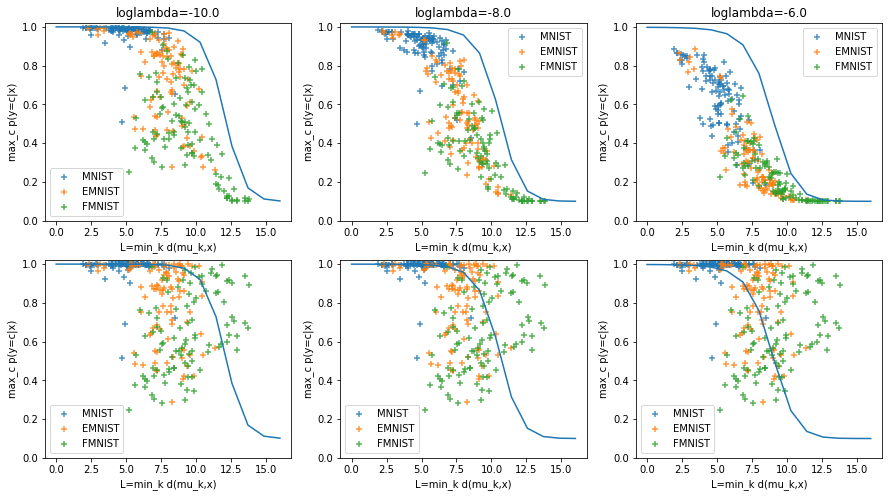
\includegraphics[width=\textwidth]{res/epsilon_L}
\caption{\label{Fig:EpsilonL} Bounds on maximum confidence as a function of the distance to the closest data point on a restricted subset of the training data for different values of $\lambda$. The centroids are located on points of this subset.}
\end{figure}

While Theorem~\ref{Thr:thr1} is true, it would be useful to have an explicit construction that allows us to infer a required distance $L$ from the training set in order to reach low confidence rather than the other way around. We achieve this with the following theorem. The assumptions are almost identical to the previous one, except now we simplify things by putting the centroids on datapoints.

\begin{theorem}\label{Thr:thr2}
Let 
$$p(y|x)=\frac{p(y|i,x)p(x|i) + \frac{\lambda}{M} }{p(x|i) + \lambda}$$
on the domain $\mathcal{D}=[0,1]^d$, where $0\leq p(y|i,x) \leq 1$, $\lambda > 0$ and $M>1$. Assume that on the domain $p(x|i)$ is given as
$$ p(x|i) = \sum_{k=0}^K \alpha_k \exp \left(-\frac{d(x,\mu_k)}{2\sigma_k^2} \right)$$
with $\alpha_k>0$, $\sigma_k^2>0$ and $\mu_k \in \mathcal{D} \quad \forall k=1,\hdots K$ and $d(\cdot,\cdot):\mathcal{D}\rightarrow [0,1]$ a metric. Furthermore let $X \subset \mathcal{D}$ and assume that $\lbrace \mu_1, \hdots, \mu_K \rbrace \subset X$.
Then for any $\epsilon > 0$ we can 
$$ \forall \epsilon >0 \forall z\in \mathcal{D}: \left( \min_{x\in X} d(z,x)=L \land L^2 \geq 2 \max_k \left( \sigma_k^2 \right) \log \left[ \frac{(M-1)\sum_k \alpha_k}{\lambda \epsilon} \right]  \right) \implies p(y|x) \leq \frac{1}{M}(1+\epsilon) $$
\end{theorem}
\begin{proof}
We can immediately see from Theorem~\ref{Thr:thr1} that a valid $L$ must exist that would satisfy the inequality. The only new part will be the explicit sufficient condition that $L$ must satisfy. We recycle from the previous proof the result
\begin{align}
p(y|x) &\leq \frac{1}{M} \frac{1 + M \frac{b}{\lambda}  }{1+\frac{b}{\lambda} } \quad \forall b\geq p(x|i)\\
b &= \sum_{k=1}^K \alpha_k \exp \left( -\frac{L^2}{2\sigma_k^2}\right) 
\end{align}
In order to write this in an adequate format for the current theorem we need an additional inequality
\begin{align}
\frac{1 + M \frac{b}{\lambda}  }{1+\frac{b}{\lambda} } &\leq 1 + (M-1) \frac{b}{\lambda}
\end{align}
This can easily be seen by noticing that $ \frac{1 + M \xi }{1+ \xi } $ is concave down, i.e.
\begin{equation}
\frac{d^2}{d \xi ^2} \frac{1+M\xi}{1+\xi} = -2\frac{M-1}{(1+\xi)^3} < 0 \quad \forall M>1, \xi>0
\end{equation}
so we can be sure that for $\xi >0$ a first order Taylor-expansion will overestimate the function. We thus find
\begin{align}
p(y|x) &\leq \frac{1}{M} \left( 1 + (M-1) \frac{b}{\lambda} \right)  \\
&= \frac{1}{M} \left( 1 + \frac{M-1}{\lambda}  \sum_{k=1}^K \alpha_k \exp \left( -\frac{L^2}{2\sigma_k^2}\right) \right) \\
&\leq \frac{1}{M} \left( 1 +  \frac{M-1}{\lambda} \left( \sum_{k=1}^K \alpha_k \right) \exp \left( -\frac{L^2}{2 \max\limits_{k} \sigma_k^2}\right) \right)\\
&\overset{!}{\leq} \frac{1}{M} \left( 1 + \epsilon \right)
\end{align}

By rearranging the last inequality we find the condition under which it applies, namely
\begin{equation}
L^2 \geq 2 \max_k \left( \sigma_k^2 \right) \log \left[ \frac{(M-1)\sum_k \alpha_k}{\lambda \ \epsilon} \right].
\end{equation}
\end{proof}

\section{Results}
Running only ACET on a plain model for 100 epochs with weight decay 5e-4 yields TE:$1.02\%$ and the following table:
\begin{tabular}{lrll}
\toprule
{} &       MMC &     AUROC &      FPR@95 \\
DataSet     &           &           &             \\
\midrule
MNIST       &  0.988259 &         - &           - \\
FMNIST      &  0.365331 &  0.996005 &        0.01 \\
EMNIST      &  0.793649 &   0.91973 &      0.3669 \\
GrayCIFAR10 &  0.103446 &  0.999991 &           0 \\
Noise       &  0.100000 &         1 &           0 \\
Adv. Noise  &  0.103789 &  0.999131 &  0.00392157 \\
Adv. Sample &  0.917343 &  0.815271 &    0.676471 \\
\bottomrule
\end{tabular}
Simply gluing a gmm with $K=1000$, initialized via EM without kmeans++, with $\log \lambda = -5$ on top yields

\begin{tabular}{lrll}
\toprule
{} &       MMC &     AUROC &    FPR@95 \\
DataSet     &           &           &           \\
\midrule
MNIST       &  0.970583 &         - &         - \\
FMNIST      &  0.344049 &  0.996876 &    0.0007 \\
EMNIST      &  0.772563 &   0.91675 &    0.2777 \\
GrayCIFAR10 &  0.101902 &  0.924797 &         0 \\
Noise       &  0.100000 &         1 &         0 \\
Adv. Noise  &  0.100000 &         1 &         0 \\
Adv. Sample &  0.904045 &  0.705438 &  0.641177 \\
\bottomrule
\end{tabular}


\end{document}
